\documentclass[article]{article}
\usepackage{lmodern}
\usepackage{setspace}
\usepackage[fleqn]{amsmath}
\usepackage{mathtools}

\usepackage[english,russian]{babel}

\usepackage{fontspec}

\setmainfont{CMU Serif}  
\setmonofont{Consolas}
\usepackage{listings}
\newfontfamily\cyrillicfonttt[Script=Cyrillic]{Consolas}

\usepackage[top=15mm, bottom=20mm, left=12mm, right=10mm]{geometry}

\usepackage{floatrow}
\usepackage[newfloat]{minted}
\usemintedstyle{manni}

\setminted[java]{
    linenos=true,
    breaklines=true,
    encoding=utf8,
    fontsize=\footnotesize,
    breaksymbol=
}
\usepackage{caption}

\usepackage{graphicx}
\usepackage[export]{adjustbox}
\usepackage{multirow}

\usepackage{amsmath}

\newenvironment{code}{\captionsetup{type=listing}}{}
\SetupFloatingEnvironment{listing}{name=Листинг}
\usepackage{tikz}
\usepackage{pgfplots}
\usepackage{filecontents}
%\usepackage{etoolbox,xpatch}
%\makeatletter
%\AtBeginEnvironment{minted}{\dontdofcolorbox}
%\def\dontdofcolorbox{\renewcommand\fcolorbox[4][]{##4}}
%\xpatchcmd{\inputminted}{\minted@fvset}{\minted@fvset\dontdofcolorbox}{}{}
%makeatother

%\begingroup
%\def\DeclareUnicodeCharacter#1#2{\setunicode{#1}#2!!}%
%\def\setunicode#1#2#3!!{%
%\ifx\undefined#2%
%  \gdef#2{\char"#1 }%
%\fi}
%\input{ot2enc.dfu}


\floatsetup[listing]{style=Plaintop, capbesideposition={top,left}}  

\onehalfspacing

\begin{document}
\begin{titlepage}
\begin{center}

\LARGE{\sc Университет ИТМО}\\~\\
\Large{\sc Факультет программной инженерии \\ и компьютерной техники}\\~\\
\Large{\sc Кафедра вычислительной техники}\\
\vfill

\Large{\sc Тестирование ПО\\ Лабораторная работа №3 \\ \emph{Вариант 999} }

\vfill
 
\hskip0.5\textwidth
\begin{minipage}{0.3\textwidth}
\begin{flushleft}

\large \emph{Выполнили:} \\  Милосердов А. О. \\ Калугин Ф. И.\\ Группа P3310

\vskip0.4in

\large \emph{Преподаватель:} \\ Клименков С. В.
\end{flushleft}

\end{minipage}
\vfill
\large Санкт-Петербург \\ \the\year  \ г.
\thispagestyle{empty}
 
\end{center}
\end{titlepage}
\captionsetup{justification=raggedright,singlelinecheck=false}
\newpage
\section*{Описание задания}
%\makebox[0pt]{}\vspace{-2ex}
Сформировать варианты использования, разработать на их основе тестовое покрытие покрытие и провести функциональное тестирование интерфейса сайта. Сайт \emph{https://tutu.ru/}.


\section*{UML -- диаграмма}
\begin{figure}[hp]
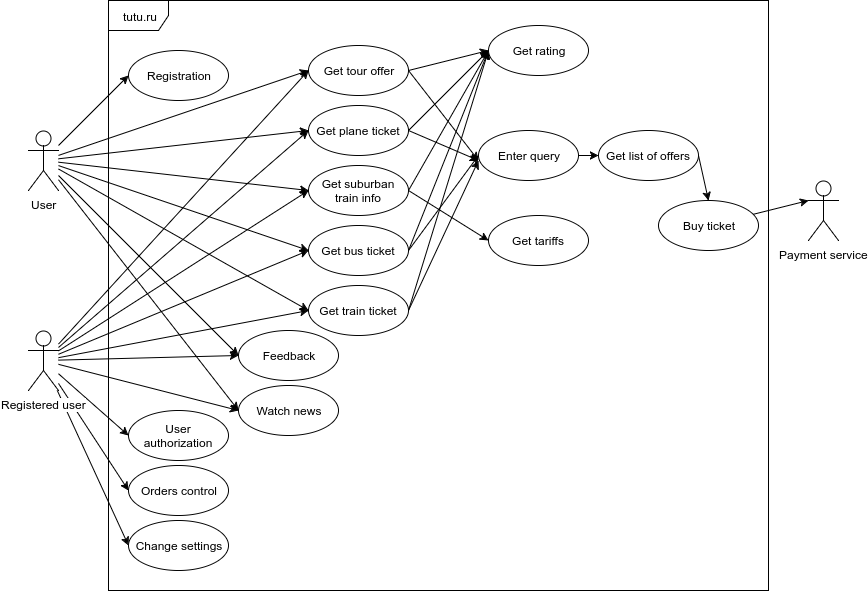
\includegraphics[width=1\textwidth]{./img/Test3UML.png}
\end{figure}

\newpage
\section*{Описание тестовых случаев}
\begin{tabular}{l|l|l|l}
\hline
	№ & Описание тестового случая & Ожидаемый результат & Статус\\
\hline
	1 & Регистрация пользователя: & Пользователь получает  & \bf{Частично:}\\
	 & 1. Пользователь заходит на страницу регистрации & аккаунт & \bf{Зарегестрированный }\\
	 & 2. Вводит данные &  & \bf{пользователь может} \\
	 & 3. Нажимает подтверждение &  & \bf{регистрироваться снова} \\
	 &  &  & \bf{при наличии id кнопки } \\
	 & & & \bf{регистрации}\\\hline
	2 & Пользователь просматривает свои заказы & - & \bf{Не тестируется}\\
\hline
	3 & Пользователь меняет свои настройки & - & \bf{Не тестируется}\\
\hline
	4 & Авторизация пользователя & - & \bf{Не тестируется}\\
\hline
	5 & Оплата билета & - & \bf{Не тестируется}\\
\hline
	6 & Обратная связь: & Сообщение об успешном & \bf{Успешно}\\
	 & 1. Открытие страницы обратной связи & запросе & \\
	 & 2. Ввод сообщения и email для связи &  & \\
	 & 3. Подтверждение &  & \\
\hline
	7 & Просмотр новостей: & Получение списка новостей & \bf{Успешно}\\
	 & 1. Нажатие на ссылку "Новости" &  & \\
\hline
	8 & Получение списка туров (для дальнейших & Получение списка & \bf{Успешно}\\
	  & выборок одинаковые шаги не повторяются): & & \\
	  & 1. Переход на страницу "Туры" & & \\
	  & 2. Ввод данных & & \\
	  & 3. Подтверждение & & \\
\hline
	9 & Получение списка билетов на поезд & Получение списка & \bf{Успешно}\\
\hline
	10 & Получение списка билетов на самолет & Получение списка & \bf{Успешно}\\
\hline
	11 & Получение списка билетов на электричку & Получение списка & \bf{Успешно}\\
	\hline
	12 & Получение списка билетов на автобус & Получение списка & \bf{Успешно}\\
\hline
	13 & Получение списка экскурсий & Получение списка & \bf{Провал: }\\
	   & & & \bf{При достаточно быстром } \\
	    & & & \bf{вводе и подтверждении} \\
	     & & & \bf{получаем 404} \\
\hline
	14 & Получить рейтинг самолета & Получить рейтинг самолета & \bf{Успешно}\\
\hline
	15 & Получить информацию о тарифах на электричку & Список тарифов  & \bf{Успешно}\\
\hline
	16 & Получить информацию о расписании  & Получение расписания & \bf{Успешно}\\
	&станции электрички &  & \\
\hline
	17 & Поиск самолета с неверными данными & Сообщение об ошибке & \bf{Успешно}\\
\hline
	18 & Переход на английскую версию сайта & Английская версия сайта & \bf{Успешно}\\
	\hline
	19 & Удаление аккаунта через настройки & Подтверждение операции & \bf{Успешно}
\end{tabular}


\end{document}
